% This is samplepaper.tex, a sample chapter demonstrating the
% LLNCS macro package for Springer Computer Science proceedings;
% Version 2.20 of 2017/10/04
%
\documentclass[runningheads]{llncs}
%
\usepackage{graphicx}
% Used for displaying a sample figure. If possible, figure files should
% be included in EPS format.
%
% If you use the hyperref package, please uncomment the following line
% to display URLs in blue roman font according to Springer's eBook style:
% \renewcommand\UrlFont{\color{blue}\rmfamily}
\usepackage{graphicx}
\usepackage{epsfig}
\usepackage{epstopdf}
\usepackage{minted}
\usemintedstyle{borland}

\epstopdfsetup{update}
\begin{document}
%
\title{Predicting product cancellations for sales retention}
%
%\titlerunning{Abbreviated paper title}
% If the paper title is too long for the running head, you can set
% an abbreviated paper title here
%
\author{Nathan Kelly\inst{1}\orcidID{0000-1111-2222-3333} \and
Hisham Ihshaish\inst{2,3}\orcidID{1111-2222-3333-4444}}
%
\authorrunning{N. Kelly Author et al.}
% First names are abbreviated in the running head.
% If there are more than two authors, 'et al.' is used.
%
\institute{Address of UWE \
\email{Hisham.Ihshaish@uwe.ac.uk}\\
\url{http://www1.uwe.ac.uk/et/csct/aboutthedepartment.aspx}}
%
\maketitle              % typeset the header of the contribution
%
\begin{abstract}
Investigate machine learning techniques to predict the likely-hood of a product cancellation based on existing sales and amount spent in annual maintenance. To enable the targeting of retention resources and offers to those customers who are predicted as at risk. 

\keywords{Sales  \and Retention \and Machine learning \and Predict \and cancellations \and Sales \and Customers}
\end{abstract}
%
%
%
\section{Background}
All businesses have problems with retention, keeping those customers they worked hard to sell to on-board when the initial excitement of the new has worn off. All too often the process of retention starts after the customer has already contacted the company to cancel. Then deep cuts in ongoing costs are offered, new features are promised and everything is reactive to the issues rather than proactive. The impact of a predictive model that can score the probability of cancellation would be that those working on retention can target the organisations directly. Proactively contacting them for information on what issues they may have and attempt to solve any problems in order to keep the sale. The added advantage is that features and issues are gleaned from the less vocal customers, the silent majority who leave with no explained reason and have a competitor lined up already.
%
%
%
\section{The training data}
\subsection{Getting the data}
The data for this study has been taken from a relational database management system (RDMS). The normalized tables have to first be joined into a single flat source. As we expect this data to be used repeatedly for ongoing model training it makes sense to create a denormalized view in the DBMS system~\cite{ref_url1}. The rows of interest from the joined tables can then be pivoted into columns for the view. This technique worked for the data in this paper, but for larger datasets the alternative of creating a flat table on a schedule or on data update can be used. The setup of this is out of the scope of this paper, but an example of the SQL used to create the dataset is provided in appendix \ref{sqlDataSource:1}. 

\subsection{Data description}
The data in the export is described below, with an example:
\begin{table}
\caption{Data description}\label{tab1}
\begin{tabular}{|l|l|l|}
\hline
Column &  Example & Description\\
\hline
\texttt{customerId} &  Id of the customer in the system & \texttt{1}\\
\texttt{amountTotal} &  Total value, in currency & \texttt{1000}\\
\texttt{salesTotal} &  Total sale value, in currency & \texttt{1000}\\
\texttt{annualTotal} &  Total annual value, in currency & \texttt{100}\\
\texttt{monthlyTotalProduct1} & Total monthly value, in currency & \texttt{10}\\
\texttt{monthlyTotalProduct2} & Total monthly value, in currency. & \texttt{10}\\
\texttt{extraItemsTotal} & Any extra items value, in currency. & \texttt{10}\\
\texttt{monthsSinceStarted} & Total number of months as customer & \texttt{15}\\
\texttt{daysToPay} & Mean number of days to pay bills & \texttt{2}\\
\texttt{creditedAmount} & Total value of credited amount, in currency & \texttt{15}\\
\texttt{isCancelled} & Boolean. Dependant variable customer cancelled product(s) & \texttt{true}\\
\texttt{hasProduct1} & Boolean, customer has product 1 & \texttt{true}\\
\texttt{...} & ... & \texttt{...}\\
\texttt{hasProduct12} & Boolean, customer has product 12 & \texttt{false}\\
\texttt{administrativeArea} & String, customer location by country admin area & \texttt{Bristol}\\
\texttt{subCountryArea} & String, customer location by sub country area & \texttt{South West}\\
\texttt{country} & String, customer location by country & \texttt{England}\\
\texttt{firstInvoiceDate} & Date ISO, first date of billing & \texttt{2018-07-08}\\
\hline
\end{tabular}
\end{table}

Column \texttt{amountTotal} is all the invoices sum'ed together. \texttt{salesTotal} is the value of each product sale combined. \texttt{annualTotal} is the recurring annual payments (if any).

Columns \texttt{hasProduct1}...\texttt{hasProduct12} represent the existence of purchased products for the company and is repeated \texttt{n} times depending on number of products sold by the company being analysied.

Column  \texttt{extraItemsTotal} contains any non product specific items sold to the customer that isn't monthly on going fees. Eg  a bundle of phone minutes at a reduced rate.

Columns \texttt{monthlyTotalProduct1} and \texttt{monthlyTotalProduct2} Represent products which have a monthly bill. In this case only product 1 and 2 have monthly bills.

\subsection{Data problems} 
Before pulling the csv file into a Jupyter notebook, it is noticed that the value for each organisation's mean time to pay in months, \texttt{monthsSincePaid} is sometimes null. This can be explained by the date the invoice was paid not being recorded. Or that the sale is new and so no paid date has yet been set. In total 14\% of the total example dataset has missing values. It makes sense to remove the new customers who have yet to pay, so the sql limits in the where clause. This still leaves null values. They will be left in the dataset and later in the paper we will compare the various imputation methods as outlined in: Missing Data: Our View of the State of the Art ~\cite{ref_url2}. It could well be that the mean value of 1 month to pay is a reasonable assumption.

\section{Feature engineering and selection}
The next step is to look at the data in the Jupyter Notebook. This is a supervised learning problem, with the discrete \texttt{isCancelled} label as our dependant variable:
\begin{figure}[ht!]
\centering
\includegraphics[width=0.7\textwidth]{dependantSpread.eps}
\caption{\label{fig:overleaf}Dependant variable spread}
\end{figure}
There are 4676 records, 2076 are customers who have cancelled a product at some point. Product 2 is the most common (2874), followed by product 1 (1878) and product 12 (1383). What the products are and do is not considered in this study, but if it was then weighting could be given to certain products at this point. For example if product 4 was a low volume high cost service or item it's status could be flagged with a categorical value. We do though have the total sale value in currency for the customer. This could be in itself enough of a weighting. The dataset is cleaned at the sql stage, a quick check for missing values gives us confidence with the data:\cite{ref_url4}:
\begin{minted}{python}
nans = lambda df: df[df.isnull().any(axis=1)]
nans(dataFrame)
\end{minted}

\subsection{Initial pipeline in sklearn}
First off, we can take our partially cleaned data from the sql source and get it in a pipeline for further investigation and processing. Using \texttt{GridSearchCV} to cross validate our training data and give us a precision score on the test split. Appendix \ref{pythonSource:2}. We'll start by dropping the catagorical features and columns \texttt{customerIdKey}, \texttt{firstInvoiceDate} to simplfy the baseline. Randomly selecting a fast classifier \texttt{LogisticRegression}. Results are:
\begin{figure}[ht!]
\centering
\includegraphics[width=0.7\textwidth]{initialScore.eps}
\caption{\label{fig:overleaf}Initial confusion matrix}
\end{figure}
\begin{minted}{python}
                precision   recall   f1-score   support

      False       0.80      0.79      0.79       859
       True       0.74      0.76      0.75       685

avg / total       0.77      0.77      0.77      1544
\end{minted}
The main score we are interested in here is the precision, our aim now is to reduce the number of false positives in the classification so we don't send our retention staff after customers who aren't going to leave.

\subsection{Categorical data}
Some of the features being ignored currently are categorical. \texttt{administrativeArea}, \texttt{subCountryArea} and \texttt{country}. A quick look at them reveals:
\begin{figure}
\centering
\includegraphics[width=0.6\textwidth]{catagoricalSubCountryArea.eps}
\caption{\label{fig:overleaf}Sub country range}
\end{figure}
\begin{figure}
\centering
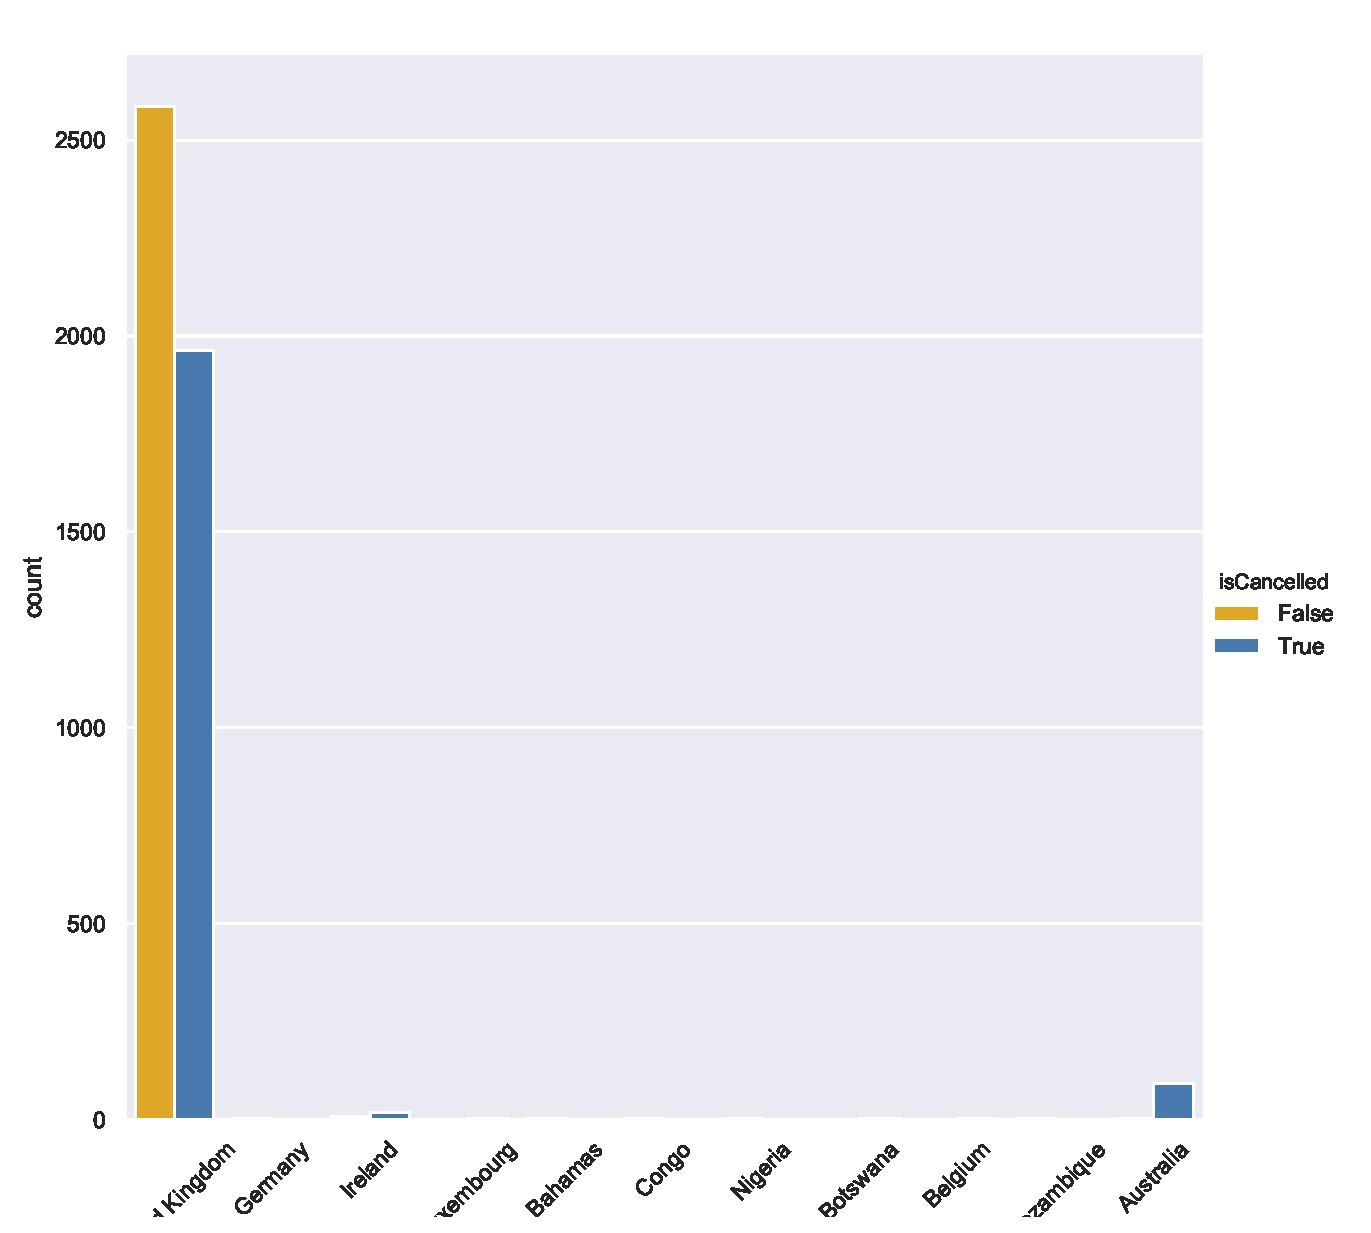
\includegraphics[width=0.6\textwidth]{catagoricalCountry.eps}
\caption{\label{fig:overleaf}Country range}
\end{figure}


\subsection{Inital feature selection}
Following the guidance in the conclusion of "An Introduction to Variable and Feature Selection" ~\cite{ref_url5}, we'll rank the features first using sklearn's \texttt{SelectKBest} method with the classification algorithms: \texttt{chi2}, \texttt{f_classif}, \texttt{mutual_info_classif}. 

Discuss cross validation and leaking of test/train datasets


%
% ---- Bibliography ----
%
% BibTeX users should specify bibliography style 'splncs04'.
% References will then be sorted and formatted in the correct style.
%
% \bibliographystyle{splncs04}
% \bibliography{mybibliography}
%
\begin{thebibliography}{8}
\bibitem{ref_url1}
Database normalization and de-normalization, \url{https://www.techrepublic.com/blog/software-engineer/code-concepts-database-normalization-and-de-normalization}. 
Last accessed 08 Jul 2018

\bibitem{ref_url2}
Joseph L. Schafer and John W. Graham: Missing Data: Our View of the State of the Art, \url{http://www.academia.edu/1045565/Missing\_Data\_Our\_View\_of\_the\_State\_of\_the\_Art}. 
Last accessed 08 Jul 2018

\bibitem{ref_url3}
A Comparative Study of Categorical Variable Encoding
Techniques for Neural Network Classifiers
\url{https://www.researchgate.net/profile/Kedar\_Potdar/publication/320465713\_A\_Comparative\_Study\_of\_Categorical\_Variable\_Encoding\_Techniques\_for\_Neural\_Network\_Classifiers/links/59e6f9554585151e5465859c/A-Comparative-Study-of-Categorical-Variable-Encoding-Techniques-for-Neural-Network-Classifiers.pdf}. Last accessed 09 Jul 201

\bibitem{ref_url4}
Python Pandas How to select rows with one or more nulls from a DataFrame without listing columns explicitly?
\url{https://stackoverflow.com/a/44702024}. Last accessed 10 Jul 2018

\bibitem{ref_url5}
An Introduction to Variable and Feature Selection
\url{http://www.jmlr.org/papers/volume3/guyon03a/guyon03a.pdf}. Last accessed 10 Jul 2018

\bibitem{ref_url6}
The importance of proper cross-validation and experimental design
\url{https://followthedata.wordpress.com/2013/10/30/the-importance-of-proper-cross-validation-and-experimental-design/}. Last accessed 23 Jul 2018

\bibitem{ref_url7}
PCA before Random Forest Regression provide better predictive scores for my dataset than just Random Forest Regression, how to explain it?
\url{https://stats.stackexchange.com/a/258945}

\bibitem{ref_article1}
Author, F.: Article title. Journal \textbf{2}(5), 99--110 (2016)

\bibitem{ref_lncs1}
Author, F., Author, S.: Title of a proceedings paper. In: Editor,
F., Editor, S. (eds.) CONFERENCE 2016, LNCS, vol. 9999, pp. 1--13.
Springer, Heidelberg (2016). \doi{10.10007/1234567890}

\bibitem{ref_book1}
Author, F., Author, S., Author, T.: Book title. 2nd edn. Publisher,
Location (1999)

\bibitem{ref_proc1}
Author, A.-B.: Contribution title. In: 9th International Proceedings
on Proceedings, pp. 1--2. Publisher, Location (2010)

\bibitem{ref_url100}
LNCS Homepage, \url{http://www.springer.com/lncs}. Last accessed 4
Oct 2017
\end{thebibliography}
\setcounter{section}{0}
\section{Appendix}
\subsection{SQL data view} \label{sqlDataSource:1}
\inputminted[
frame=lines,
fontsize=\footnotesize,
]{sql}{sqlData.sql}

\subsection{Python initial pipeline view} \label{pythonSource:2}
\inputminted[
frame=lines,
fontsize=\footnotesize,
]{python}{initialPipeline.py}
\end{document}
